\chapter{Upper and lower bounds of the design variables}%
\label{app:A}

% Upper and lower bounds used in the optimization problem consisting of the initial conditions for the knee and hip angles of the swing leg,$~q_{5,~IC}$ and$~q_{4,~IC}$, the angle of the torso$~q_{3,~IC}$, their corresponding velocities$~\dot{q}_{5,~IC}$,$~\dot{q}_{4,~IC}$ and$~\dot{q}_{3,~IC}$ as well as$~\gls{lambda}_{IC}$, the initial angle of~\gls{v}$_{\glsxtrshort{com}}$, are shown in table~\ref{tab:upper-and-lower-bounds}.

\begin{table}[H]
    \caption{Upper and lower bounds used in the optimization problem consisting of the initial conditions for the knee and hip angles of the swing leg,$~q_{5,~IC}$ and$~q_{4,~IC}$, the angle of the torso$~q_{3,~IC}$, their corresponding velocities$~\dot{q}_{5,~IC}$,$~\dot{q}_{4,~IC}$ and$~\dot{q}_{3,~IC}$ as well as$~\gls{lambda}_{IC}$, the initial angle of~\gls{v}$_{\glsxtrshort{com}}$.} 
    \label{tab:upper-and-lower-bounds}
    \begin{center}
        \begin{tabular}{ l|l|l|l|l }
            \textbf{Symbol}                 & \textbf{Description}                      & \textbf{Lower bound}  & \textbf{Upper bound}  & \textbf{Unit}                          \\ [0.5ex]
            \hline \hline
            $q_{5,~IC}$               & Angle of the right knee                   & $-110$                & $-10$                 &$~\left[\si{\degree}\right]$            \\
            $q_{4,~IC}$               & Angle of the right hip                    & $-70$                 & $70$                  &$~\left[\si{\degree}\right]$            \\
            $q_{3,~IC}$               & Angle of the torso                        & $-20$                 & $20$                  &$~\left[\si{\degree}\right]$            \\
            $\gls{lambda}_{IC}$             & Angle of~\gls{v}$_{\glsxtrshort{com}}$    & $-30$                 & $30$                  &$~\left[\si{\degree}\right]$            \\
            $\dot{q}_{5,~IC}$         & Angular velocity of the right knee        & $-3$                  & $3$                   &$~\left[\si{\radian\per\second}\right]$ \\
            $\dot{q}_{4,~IC}$         & Angular velocity of the right hip         & $-3$                  & $3$                   &$~\left[\si{\radian\per\second}\right]$ \\
            $\dot{q}_{3,~IC}$         & Angular velocity of the torso             & $-3$                  & $3$                   &$~\left[\si{\radian\per\second}\right]$ \\
        \end{tabular}
    \end{center}
\end{table}
% \noindent
%

\chapter{Vertical velocity of the center of mass}%
\label{app:B}

\begin{figure}[htb]%
    \centering%
    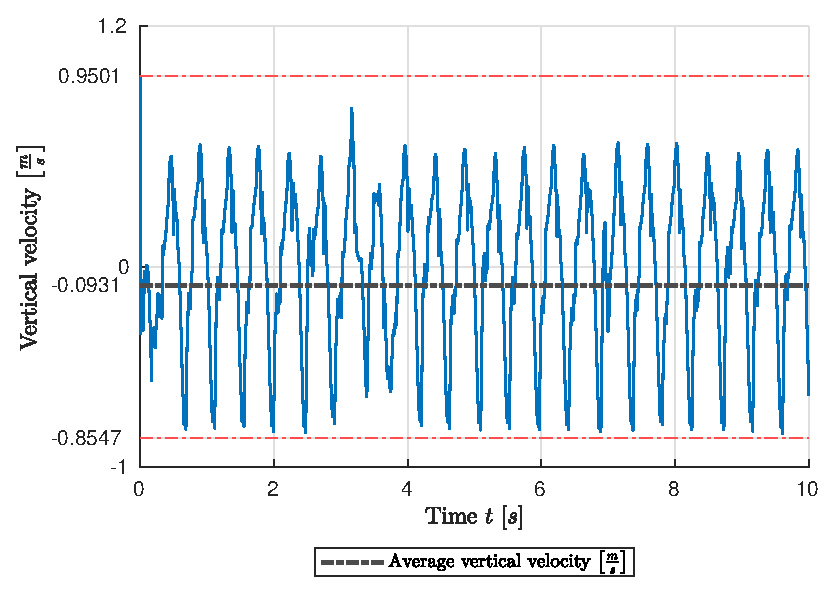
\includegraphics[width=\linewidth]{com-velocity/com-vertical-velocity.eps}
    \caption{The trajectory of the vertical velocity of the~\glsxtrlong{com} during the motion. For legibility purposes, the first $10\,\textrm{\si{\second}}$ of movement are displayed. The average vertical velocity is $-0.0931\,\textrm{\si{\metre\per\second}}$. The amplitude of the vertical velocity ranges from a maximum of $0.9501\,\textrm{\si{\metre\per\second}}$ to a minimum of $-0.8547\,\textrm{\si{\metre\per\second}}$.}%
    \label{fig:com-vertical-velocity}%
\end{figure}%
% \noindent
